\chapter{Модальное управление по выходу}
\label{ch:chap3}
\section{Условие задачи}

Рассматриваем систему:
$$
  \begin{cases}
    \dot{x} = Ax + Bu\\
    y = Cx + Du
  \end{cases}
$$ и выполнить следующие шаги:
  \begin{itemize}
  \item  Найти собственные числа матрицы $A$ и определить наблюдаемость каждого из них. 
   Сделать вывод об наблюдаемости и обнаруживаемости системы.
  \item  Построить схему моделирования системы, замкнутой регулятором, состоящем
    из наблюдателя состояния  и закона управления.
  \item  Задаться парой достижимых желаемых спектров для регулятора и наблюдателя,
  обеспечивающих асимптотическую устойчивость замкнутой системы.
  \item Синтезировать регулятор $K$ на основании выбранного желаемого спектра, определить
    собственные числа матрицы $(A+BK)$ и сравнить с желаемым спектром
  для проверки корректности расчетов.
  \item Синтезировать матрицу коррекции наблюдателя $L$ на основании выбранного желаемого спектра, 
  определить собственные числа матрицы $(A +LC)$ и сравнить с
  желаемым спектром для проверки корректности расчетов.
  \item  Выполнить компьютерное моделирование с начальными условиями системы 
  $x(0) = \begin{bmatrix} 1&1&1&1 \end{bmatrix}^T$ и наблюдателя $\hat{x}(0)=\begin{bmatrix}0 & 0& 0 &0\end{bmatrix}^T $.
  Построить  сравнительные графики $x(t)$ и $\hat{x}(t)$, график управления $u(t)$ и ошибки наблюдателя
   $e(t) = x(t) - \hat{x}(t)$
  \end{itemize}
      
\section{Решение задачи}

Параметры для объекта:
$$
  A = \begin{bmatrix}
    5  &  -7   & -5  &   1 \\
   -7   &  5  &  -1   &  5 \\
   -5  &  -1  &   5   &  7 \\
    1  &   5  &   7   &  5

  \end{bmatrix} \tab
  B = \begin{bmatrix}
    5\\7\\1\\9
  \end{bmatrix} \tab
  C = \begin{bmatrix}
    0 & 0 & 2 & 2\\
    1 & 1 & -1 & -1
  \end{bmatrix} \tab
  D = \begin{bmatrix}
    4\\2
  \end{bmatrix} 
$$



\subsection{Исследование наблюдаемости системы}
Для начала найдём матрицу наблюдаемости системы:
$$
V = \begin{bmatrix}
    C \\ CA \\ CA^2
\end{bmatrix} = \begin{bmatrix}
                1   &	0	&  2 \\
                4   &   -3  &  2 \\
                -11  &    -6  &  16
            \end{bmatrix}
$$
$$
  rank(V) = 3
$$
По критерию Калмана, наша система полностью наблюдаема , так как ранк матрицы наблюдаемости равен порядку системы.

Найдём собственные числа матрицы $A$:
$$
    \sigma(A) = \{-8, 4, 8, 16\}
$$
\subsection{Синтез наблюдателя и регулятора}
Выберем следующие два спектра для наблюдателя и регулятора, которые обеспечат асимптотическую устойчивость замкнутой системы:
$$
    \sigma(G_{ctrl}) = \{-1, -4, -4, -4\}, \tab \sigma(G_{obsv}) = \{-1, -3, -3, -3\}
$$
Пользуясь упомянутомы методома синтеза регулятора и наблюдателя через уравнения Сильвестра, получим следующие матрицы $K, L$:
$$
G_{ctrl} = \begin{bmatrix}
  -1  &   0  &   0  &   0 \\
  0  &  -4   &  1   &  0 \\
  0  &   0  &  -4  &   1 \\
  0   &  0   &  0  &  -4
\end{bmatrix}, \tab Y = \begin{bmatrix} 1\\1\\1\\1 \end{bmatrix}^T, \rightarrow 
K = \begin{bmatrix} 8.51 \\ -8.91 \\ -0.87 \\ -1.36 \end{bmatrix}^T
$$
$$
G_{obsv} = \begin{bmatrix}
  -1  &   0  &   0  &   0 \\
  0  &  -3   &  1   &  0 \\
  0  &   0  &  -3  &   1 \\
  0   &  0   &  0  &  -3
\end{bmatrix}, \tab Y = \begin{bmatrix}1&1\\1&1\\0&0\\1&1\end{bmatrix},\rightarrow
L = \begin{bmatrix}
  35.60 & 35.60\\
 -38.39 & -38.39\\
 -12.02 & -12.02\\
 -15.18 & -15.18
\end{bmatrix}
$$
Теперь вычислим собственные числа матрицы регулятора $(A+BK)$ и наблюдателя $(A+LC)$:
$$
    \sigma(A+LC) = \{-1, -3.0005, -2.9997 \pm 0.0004i\}
$$
$$
  \sigma(A+BK) = \{-1, -3.9996   -4.0002 \pm 0.0004i\}
$$
Спектры почти совпали с точностью до погрешности, значит синтез корректен в обеих случаях.
\newpage
\subsection{Моделирование}
Выполним  моделирование с начальными условиями системы 
  $x(0) = \begin{bmatrix} 1&1&1&1 \end{bmatrix}^T$ и наблюдателя $\hat{x}(0)=\begin{bmatrix}0 & 0& 0 &0\end{bmatrix}^T $,

  Построим следующие графики:
  \begin{figure}[ht]
    \centering
    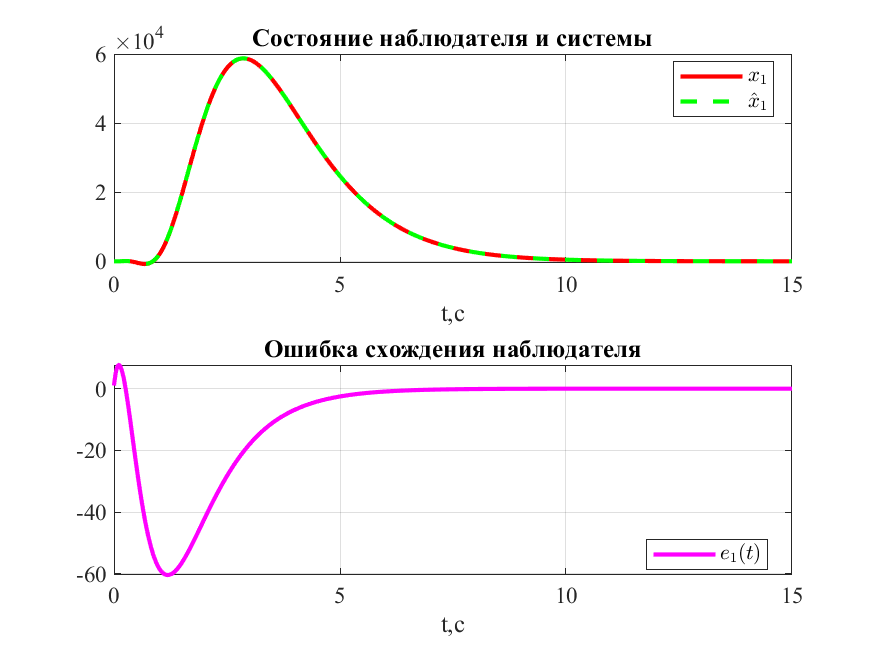
\includegraphics[width=0.8\textwidth]{obsv_ctrl1.png}
    \caption{Состояние системы и ошибка сходимости}
  \end{figure}
  \newpage
  \begin{figure}[ht]
    \centering
    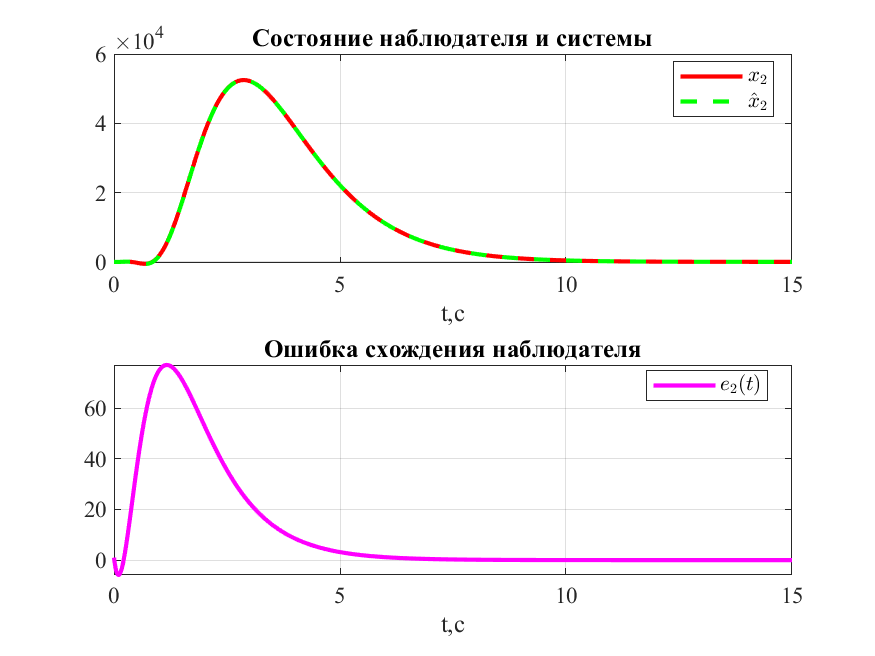
\includegraphics[width=0.8\textwidth]{obsv_ctrl2.png}
    \caption{Состояние системы и ошибка сходимости}
  \end{figure}
  \begin{figure}[ht]
    \centering
    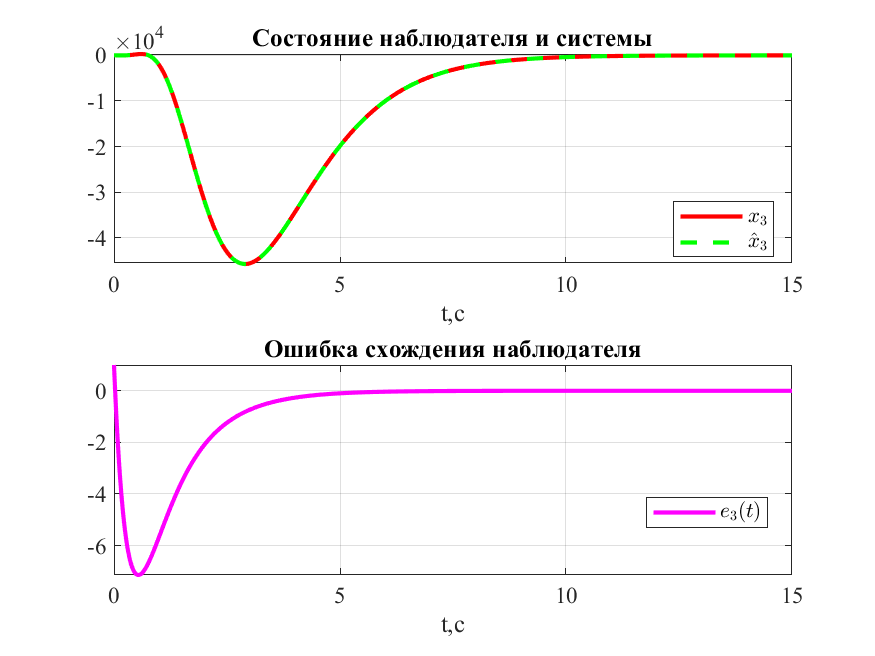
\includegraphics[width=0.8\textwidth]{obsv_ctrl3.png}
    \caption{Состояние системы и ошибка сходимости}
  \end{figure}
  \newpage
  \begin{figure}[ht]
    \centering
    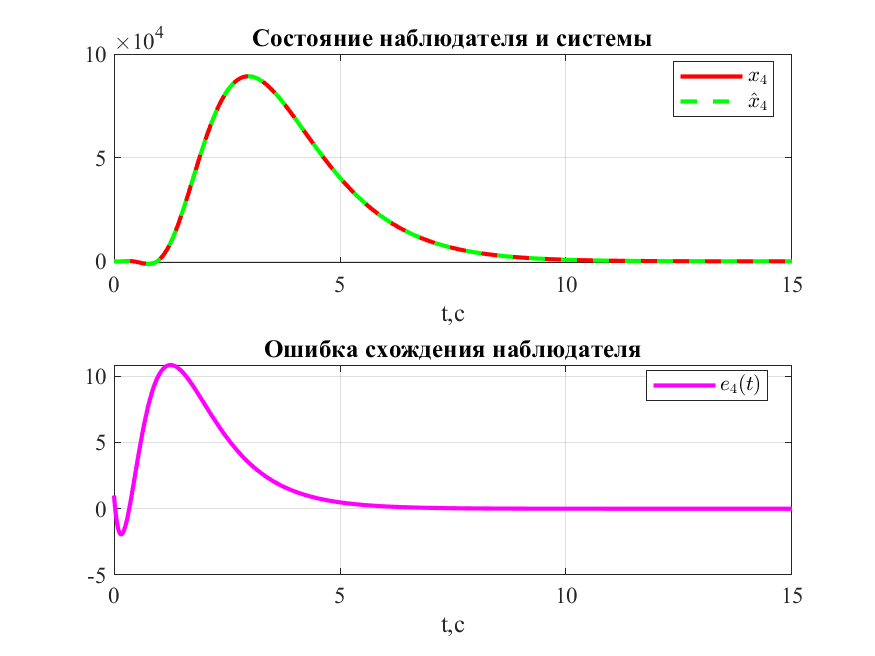
\includegraphics[width=0.8\textwidth]{obsv_ctrl4.png}
    \caption{Состояние системы и ошибка сходимости}
  \end{figure}
  \begin{figure}[ht]
    \centering
    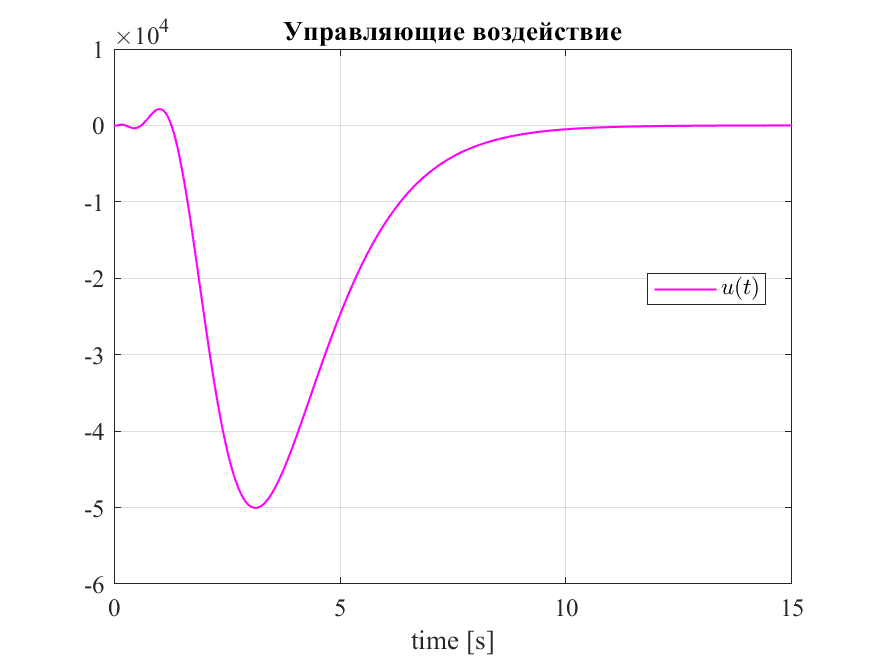
\includegraphics[width=0.8\textwidth]{obsv_ctrl_u1.png}
    \caption{Управление регулятора}
  \end{figure}

\newpage
\subsection{Вывод}
В этом задании мы синтезировали полное управление по выходу - связку наблюдателя и регулятора. 
В этот раз мы работали с полностью наблюдаемой и управляемой системой, поэтому мы могли использовать любой желаемый спектр у наблюдателя/регулятора.
Моделирование показало, что связка отработала успешно.

\endinput